\section{Comparisons}
In order to compare the two pareto fronts in the results above, each design was exposed to an identical load consisting of a 147 kN force acting vertically along the y axis. The peak stress was obtained and tabulated. 

\subsection{Comparison of Long Run Results}
Figure \ref{fig:pfront_comp_long} shows a plot of this compairson between the two Long-Run fronts. Note that the solver for the aggregate LHS appears to cover a wider portion of the solution space, but that both graphs follow roughly the same curve. 

\begin{figure}[!htbp]
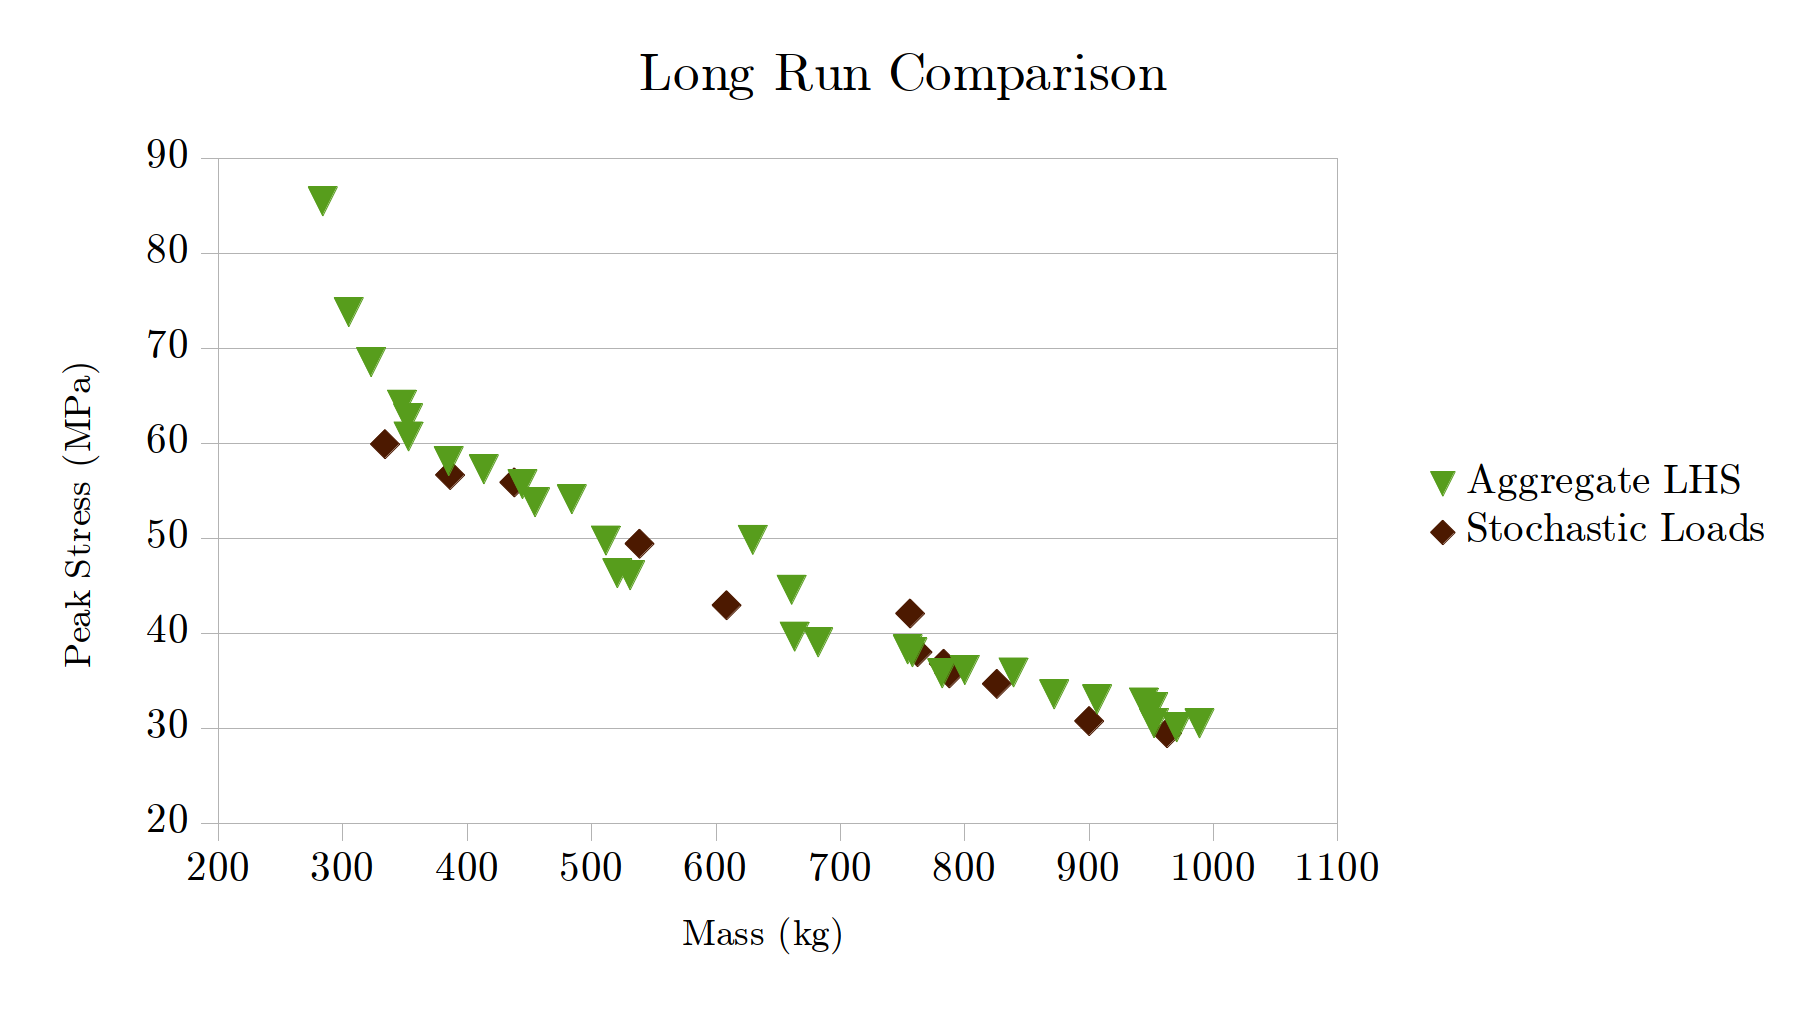
\includegraphics[width=\textwidth]{img/pf_comp_long.png}
\caption{Comparison of the Two Long Run Pareto Plots}
\label{fig:pfront_comp_long}
\end{figure}

\subsection{Comparison of Short Run Results}
Figure \ref{fig:pfront_comp_short} shows a plot of this compairson between the two Short-Run fronts. Note that despite the same solution times, the Stocastic Loads plot has resulted in designs returning higher stress values in some weight ranges. 

\begin{figure}[!htbp]
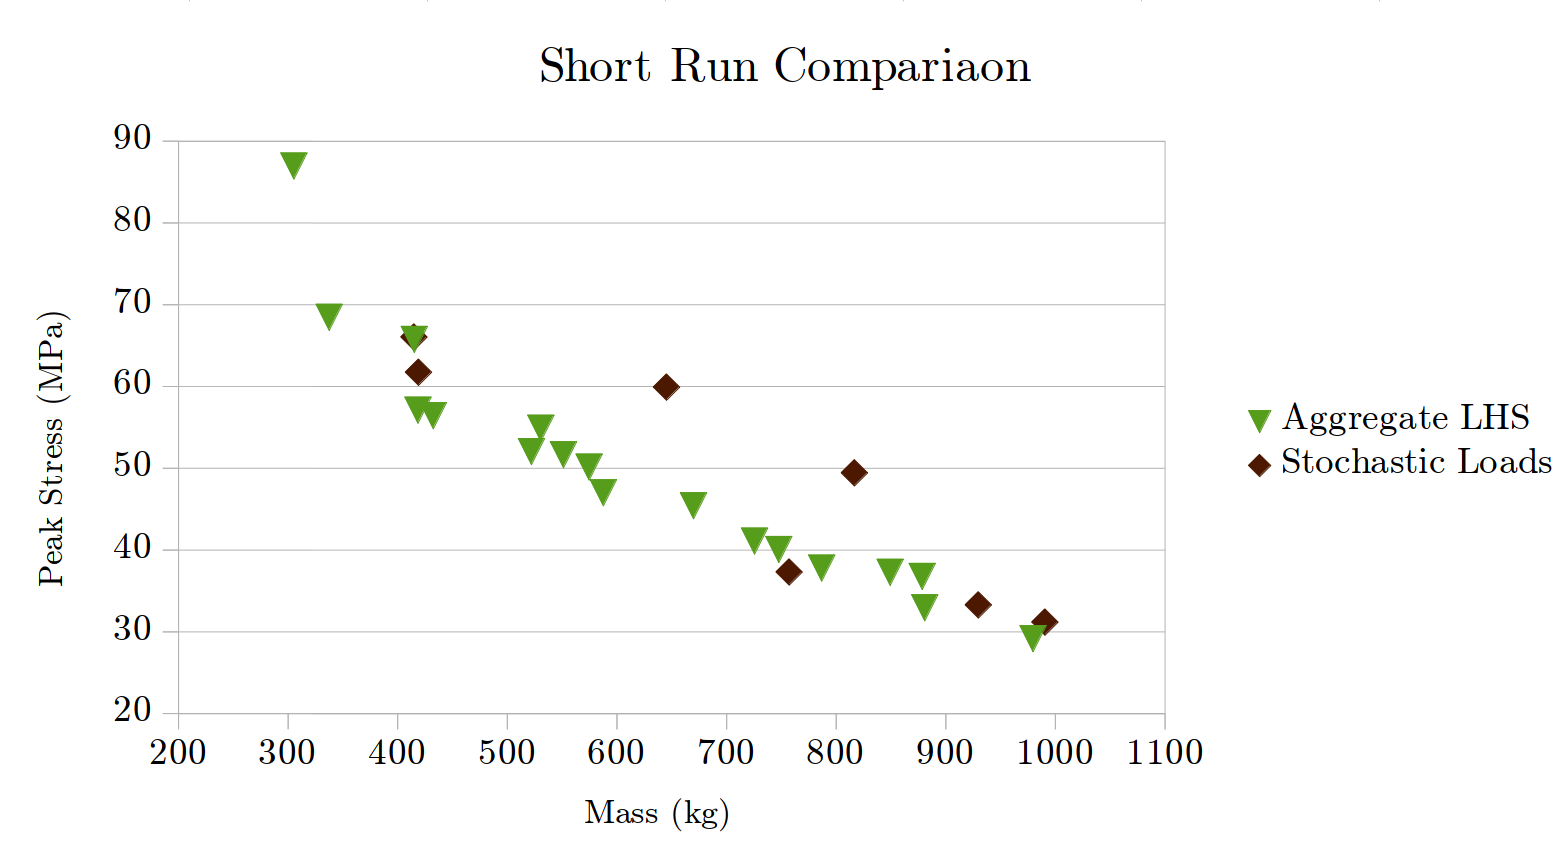
\includegraphics[width=\textwidth]{img/pf_comp_short.png}
\caption{Comparison of the Two Short Run Pareto Plots}
\label{fig:pfront_comp_short}
\end{figure}
